\section{TESTS}

\subsection{Results Summary}

After completion of all testing, no IPCs dropped any messages during transit. This can be attributed to the ideal testing conditions. Hardwired network communication and single byte package size allowed for both TCP and UDP packets to be received despite UDP's lower inherenit reliability. The introduction of a wireless networks or lower quality routers may cause more of a differentiation to arise. The fastest overall system consisted of UDP network messages and ACH messages for the internal communication through the Pi. There was negligable difference in transit time between TCP and UDP over the network. Similar delays at this stage of the test can be attributed to the routers throughput. TCP response messages are processed at or below the microsecond accuracy level and does not impact our test results. A summary of all data collected is presented below for the network link in Table \ref{table:results summary net} and the internall Raspberry Pi link in Table \ref{table:results summary rpi}.

\begin{table}[h]
\caption{Results Summary: Network Link}
\label{table:results summary net}
\begin{center}
\begin{tabular}{c|c||c||c||c||c|}
\cline{2-6}
& \multicolumn{5}{c|}{Network: Link 1}\\
\hline
\multicolumn{1}{|c|}{Item} & UDP & TCP & ZMQ &ACH & ROS\\
\hline
\multicolumn{1}{|c|}{Average (ms)} & 3.834 & 3.829 & 5.285 & N/A & 13.09\\
\hline
\multicolumn{1}{|c|}{Min (ms)} & 3.359 & 3.399 & 3.943 & N/A & 4.860\\
\hline
\multicolumn{1}{|c|}{Max (ms)} & 95.063 & 42.006 & 92.746 & N/A & 706.840\\
\hline
\multicolumn{1}{|c|}{Std Deviation (ms)} & 1.441 & 0.768 & 3.639 & N/A & 1.292\\
\hline
\end{tabular}
\end{center}
\end{table}

\begin{table}[h]
\caption{Results Summary: Raspberry Pi Link}
\label{table:results summary rpi}
\begin{center}
\begin{tabular}{c|c||c||c||c||c|}
\cline{2-6}
& \multicolumn{5}{c|}{Raspberry Pi: Link 2}\\
\hline
\multicolumn{1}{|c|}{Item} & UDP & TCP & ZMQ & ACH  & ROS\\
\hline
\multicolumn{1}{|c|}{Average (ms)} & 3.834 & 4.774 & 5.000 & 3.752 & 17.571\\
\hline
\multicolumn{1}{|c|}{Min (ms)} & 3.359 & 4.079 & 3.853 & 3.219 & 5.680\\
\hline
\multicolumn{1}{|c|}{Max (ms)} & 95.063 & 43.974 & 161.833 & 73.533 & 709.943\\
\hline
\multicolumn{1}{|c|}{Std Deviation (ms)} & 1.441 & 1.160 & 3.171 & 1.705 & .9958\\
\hline
\end{tabular}
\end{center} 
\end{table}

\subsection{UDP Results (Control)}

The control of this experiment utilized UDP messages over the network and UDP messages sent to the loopback address on the Pi. No missed messages occured despite UDP being the least reliable IPC method tested. Consistent results occured with a standard deviation of 1.441 ms and the average transit was 3.834 ms. This was the second fastest configuration tested. Figure \ref{fig:UDP results} below shows a summary of collected data with outliers removed for clarity.

\begin{figure}[thpb]
 \centering
 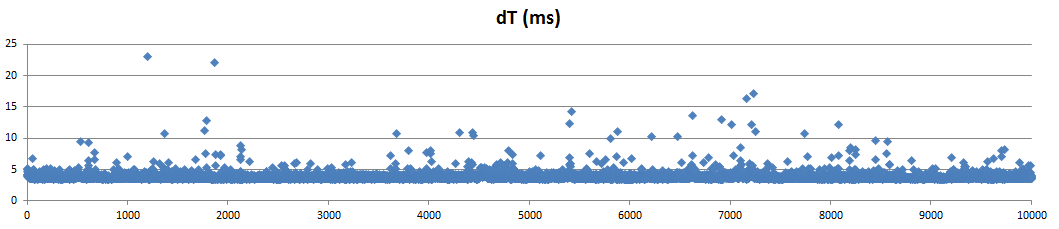
\includegraphics[width=1.0\columnwidth]{./images/udp2udp.png}
  \caption{UDP Control Test Results}  
  \label{fig:UDP results}
\end{figure} 

\subsection{TCP Results}

TCP was tested in both Link 1 and Link 2 configurations with UDP as the second link. No missed messages were recorded as expected for TCP. For the network link, TCP performed with negligable difference to UDP. This would suggest that for small data packets and reliable network connections the additional delay incurred by TCP's response message is negligable. Figure \ref{fig:TCP L1 results} below shows a summary of collected data with outliers removed for clarity.

\begin{figure}[thpb]
 \centering
 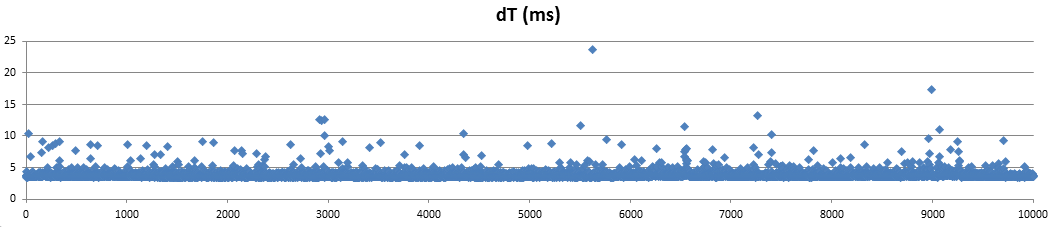
\includegraphics[width=1.0\columnwidth]{./images/tcp2udp.png}
  \caption{TCP Link 1 Test Results}  
  \label{fig:TCP L1 results}
\end{figure} 

Differentiation arises when TCP is utilized for the Link 2 loopback transport. Additional latency was recorded for an averate transit time of 4.774 ms and a standard deviation of  1.160 ms. This suggests the additional TCP overhead becomes an issue for embedded systems and would not be a valid candiate for an internal IPC. Figure \ref{fig:TCP L2 results} below summarizes the Link 2 test results.

\begin{figure}[thpb]
 \centering
 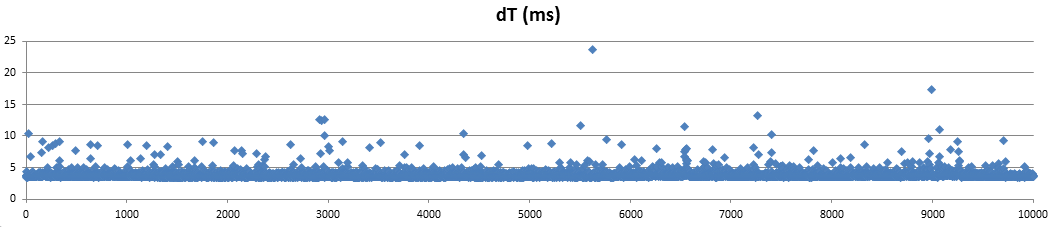
\includegraphics[width=1.0\columnwidth]{./images/tcp2udp.png}
  \caption{TCP Link 2 Test Results}  
  \label{fig:TCP L2 results}
\end{figure} 

\subsection{ZMQ Results}

ZeroMQ performed the slowest in both links of all the pure IPCs tested. It is expected that ZMQ performs slower than TCP as it includes additional packet information around a standard TCP message. This test only determines the speed of a single process communicating in client/server pair and does not evaluate potential gains when implemented in a multifaceted topology. ZMQ was tested in both Link 1 and Link 2 configurations and results can be found below in Figure \ref{fig:ZMQ L1 results} (Link 1) and Figure \ref{fig:ZMQ L2 results} (Link 2) below.

\begin{figure}[thpb]
 \centering
 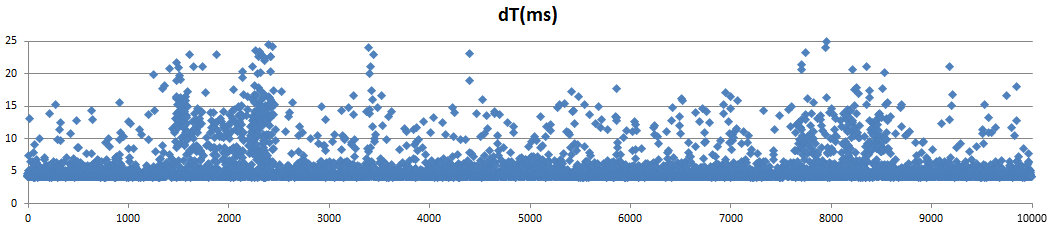
\includegraphics[width=1.0\columnwidth]{./images/zmq2udp.png}
  \caption{ZMQ Link 1 Test Results}  
  \label{fig:ZMQ L1 results}
\end{figure} 

\begin{figure}[thpb]
 \centering
 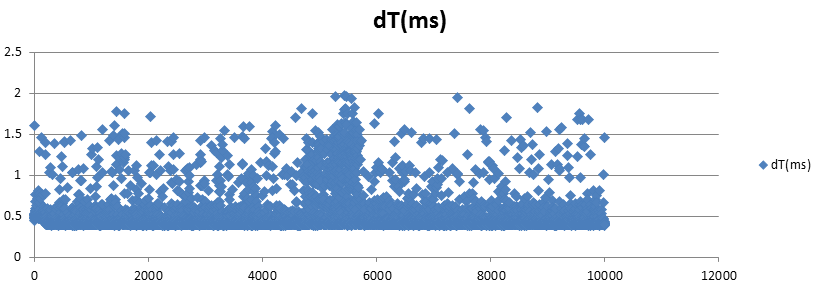
\includegraphics[width=1.0\columnwidth]{./images/udp2zmq.png}
  \caption{ZMQ Link 2 Test Results}  
  \label{fig:ZMQ L2 results}
\end{figure} 

The data shows slower performance in both link configurations than UDP, TCP, or ACH. Certain peroids of increased latency were observed and could be a result of messaging speed and increased overhead of ZMQ overwhelming the SBC for short durations. If ZMQ would be implemented for all links in a system, the delay would be compounded with each step.

\subsection{ACH Results}

ACH performed the fastest of all IPC methods tested. For consistency, UDP was used as the Link 1 transport over the ACHD library. ACHD can be configured as TCP or UDP messages and it was concluded that similar results would have been produced. Average transit time was 3.752 ms with a standard deviation of 1.705 ms. ACH exceeds the speed of UDP when transmitting internally and has the synchronization benefits of ZMQ without the additional latency observed. Figure \ref{fig:achresults} below shows a summary of collected data with outliers removed for clarity.

\begin{figure}[thpb]
 \centering
 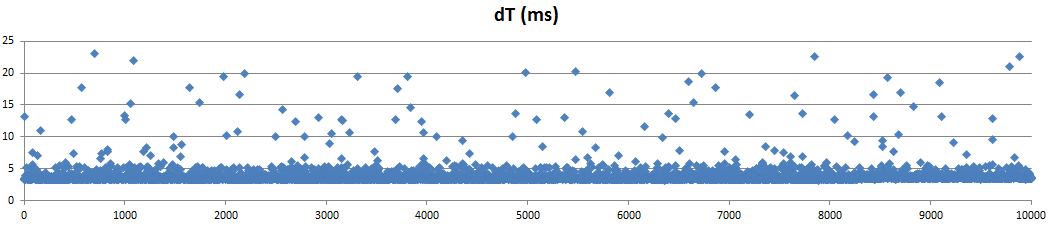
\includegraphics[width=1.0\columnwidth]{./images/achtest.png}
  \caption{ACH L2 Test Results}  
  \label{fig:achresults}
\end{figure} 

\subsection{ROS Results}

ROS performed the slowest of all IPC methods tested. The test of link 1 was performed by running a ROScore instance on the full computer and a publish/subscribe link built between each process in the communication path. Running the ROScore on the networked computer introduced additional latency from network communications, but freed up processing power on the SBC. This test incorporates ROS messages in both link 1 and link 2 as it is the more logical implementation for a fully networked ROS system. The additional overhead of ROS messages and the extra communications with the ROScore process substantially impacted latency. Results can be found below in Figure \ref{rosfull}.

\begin{figure}[thpb]
 \centering
 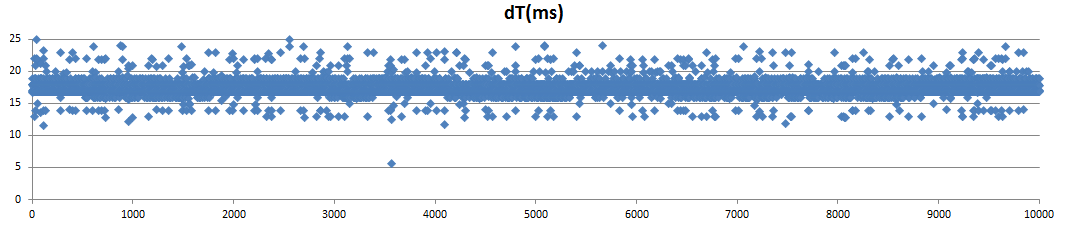
\includegraphics[width=1.0\columnwidth]{./images/rosfull.png}
  \caption{ROS Full Network Test Results}  
  \label{fig:rosfull}
\end{figure} 

To futher test the impact of ROScore on the system. A link 2 test was established to simulate a fully contained ROS system on the SBC with UDP communications over the network. Increased latency was recorded despite the fewer messages to a remote ROScore. This indicates that for embedded sytems, the increased procressing power required to run ROScore is detrimental to the operation of the robot. Results are found below in Figure \ref{roslink2}.

\begin{figure}[thpb]
 \centering
 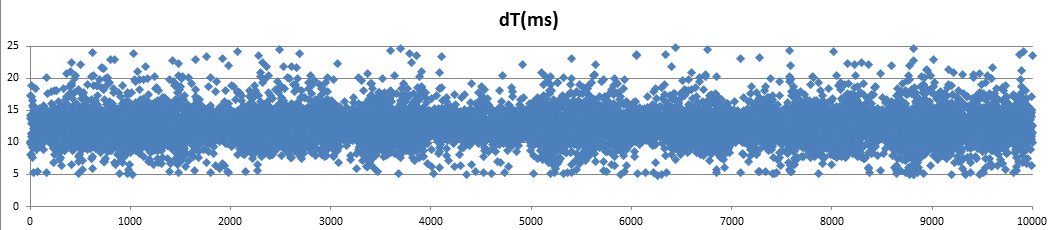
\includegraphics[width=1.0\columnwidth]{./images/roslink2.png}
  \caption{ROS Link 2 Test Results}  
  \label{fig:rosfull}
\end{figure} 


